\section{Implementation}\label{sec:impl}
\begin{newpart}{MK@Tom: this is your's, I am just giving some first text}
  The implementation of in-situ computation is organized along the information model
  outlined in the last section. It is realized as a Javascript module in the JOBAD
  framework~\cite{JOBAD:on}, a Javascript for instrumenting (active) documents with user
  interactions; see~\cite{GLR:WebSvcActMathDoc09} for details.

  A right click on a formula $F$ triggers the JOBAD menu, which has a ``compute with me''
  field, which triggers
  \begin{itemize}
  \item The \textbf{context extractor}, a function that for all the \lstinline|ci|
    elements in the content formula $C$ associated with $F$, tries to find the associated
    variable declarations by going up the parent chain of $F$ and the symbol declarations
    from the home theory -- the latter is functionality provided by the MMT system. Note
    that using the content MathML representation $C$ of $F$ gets us around disambiguation
    problems: even if the presentation of $F$ is ambiguous (e.g. by using variable or
    constant names multiple times), $C$ is not.
  \item The variable context is displayed to the user prompting instantiation in a popup
    form: the \textbf{in-situ computation manager} (see Figure~\ref{fig:compman}\ednote
    {replace this with a screenshot.}), which allows to give values for the components of
    the equation, specify actions (simplification, equation solving, \ldots) and ways of
    providing the results.\ednote{MK: we should think of more ways than ``in-place'' and
      ``footnote'' here.}\ednote{MK: the manager should eventually also give access to
      multiple computation machines.}
  \item The user-supplied values are parsed into Content MathML, inserted into $C$,
    yielding the content MathML expression $C'$, which is then shipped to the
    computational engine. Currently we only support the MMT system as a computational
    engine, but this is not a restriction, since MMT can delegate computations to engines
    like GAP, Sage, PARI, \ldots via the SCSCP protocol~\cite{ODK-D3.3}. 
  \item Finally, the result $R$ of computing $C'$ -- a content MathML expression -- is
    presented in presentation MathML and inserted into the document. \ednote{show screen
      shots of the examples from Section~\ref{sec:examples}.}
  \end{itemize}

  \begin{figure}[ht]\centering
    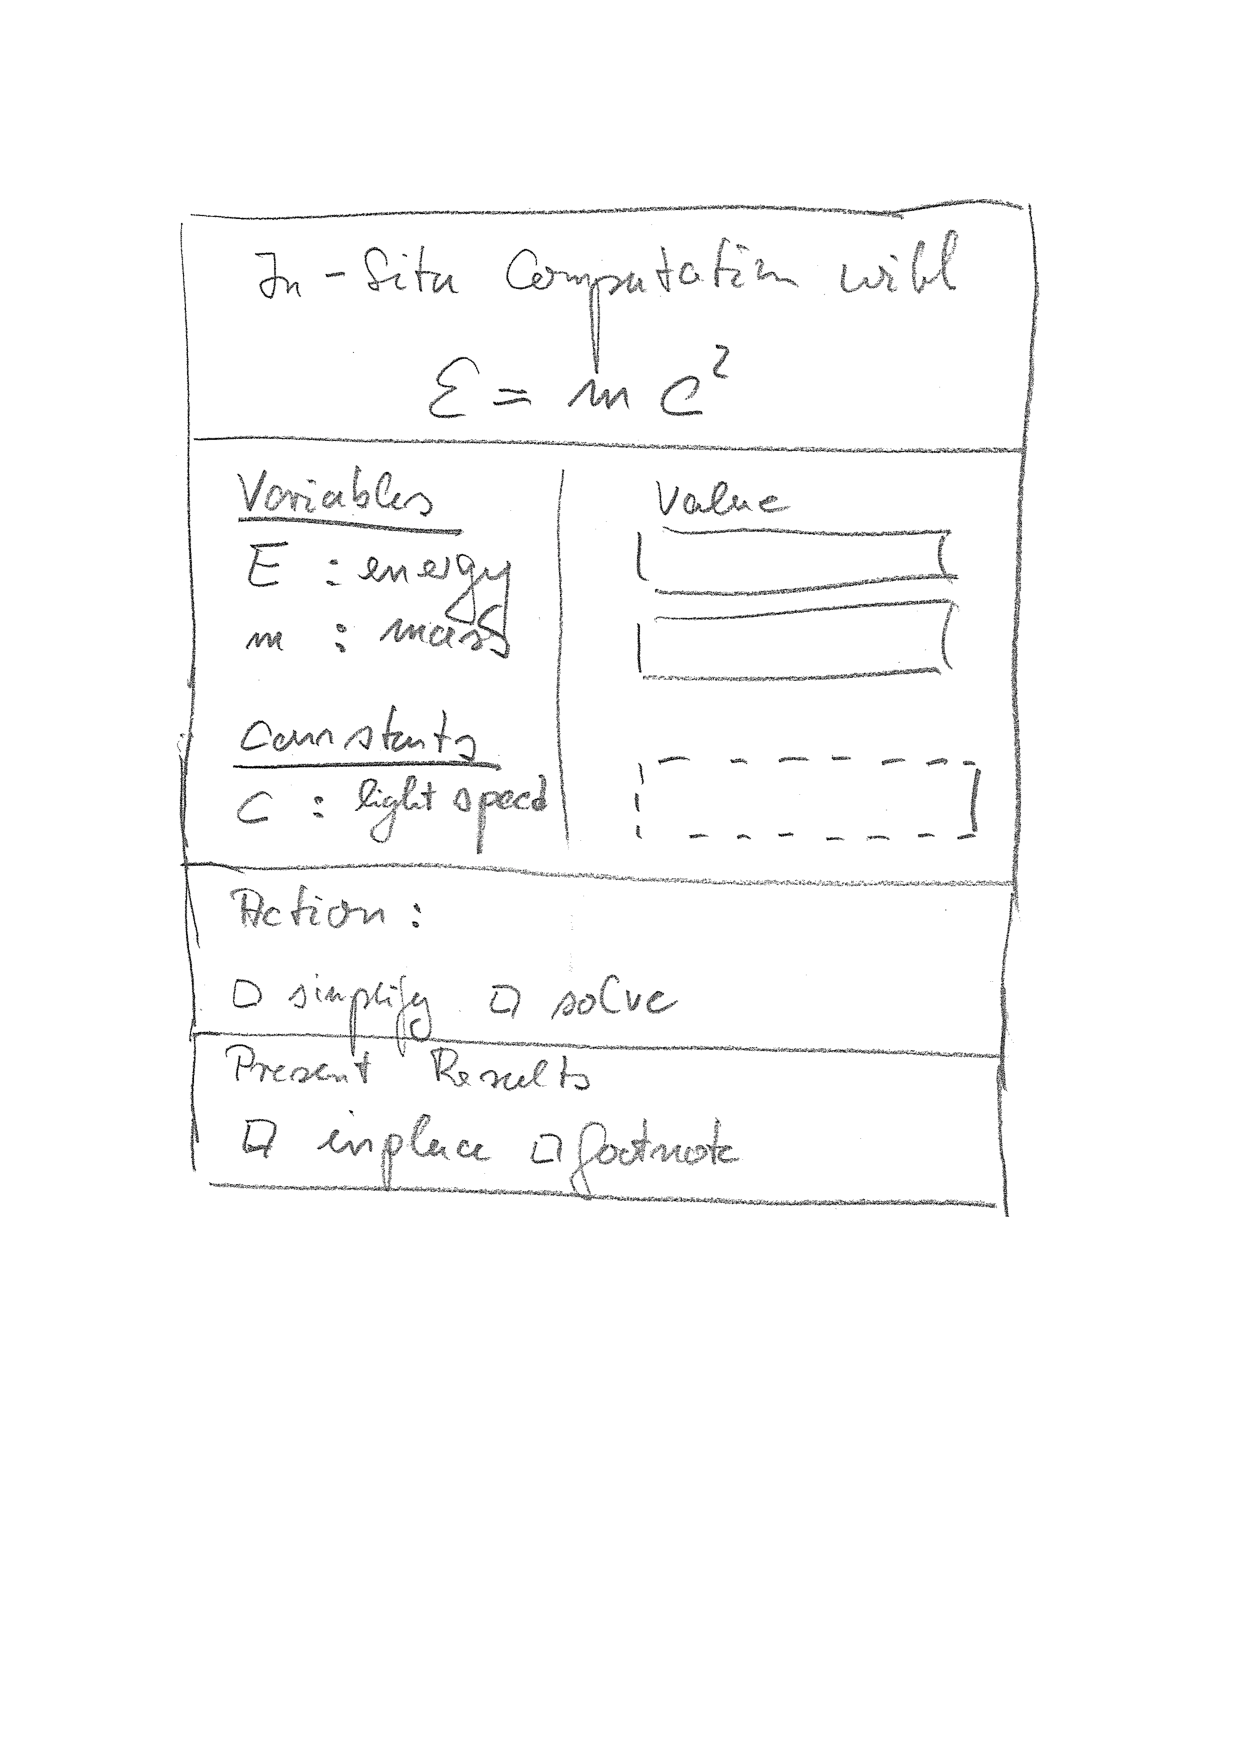
\includegraphics[width=10cm]{compman}
    \caption{In-Situ Computation Manager}\label{fig:compman}
  \end{figure}

  
  \subsection{Unit Conversion}
In this section we will describe two use cases for automatic unit conversions, both of which
are already implemented using the JOBAD framework.

Before starting to convert something, the user can highlight all quantity
expressions in a given document. This results in a document, as shown in
Figure~\ref{fig:highlight}. We further use this snippet as running example.

\begin{figure}
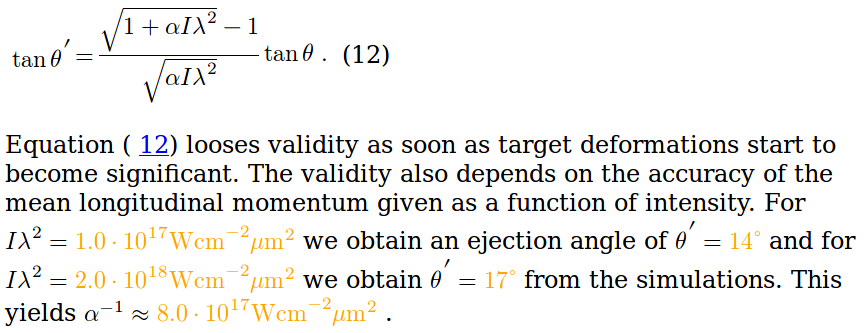
\includegraphics[scale=0.3]{screenshots/highlight.png}
\caption{An example of a document, where the quantity expressions are highlighted.}
\label{fig:highlight}
\end{figure}

In the first case, the user wants to convert a unit in just one expression to
an equivalent one, say watt to horsepower. For that, he can rightclick on this
particular expression and choose horsepower from the list of units that are
equivalent to watt. Figure~\ref{fig:convertone} demonstrates this and
Figure~\ref{fig:convertoneresult} displays the result of the computation. 

\begin{figure}
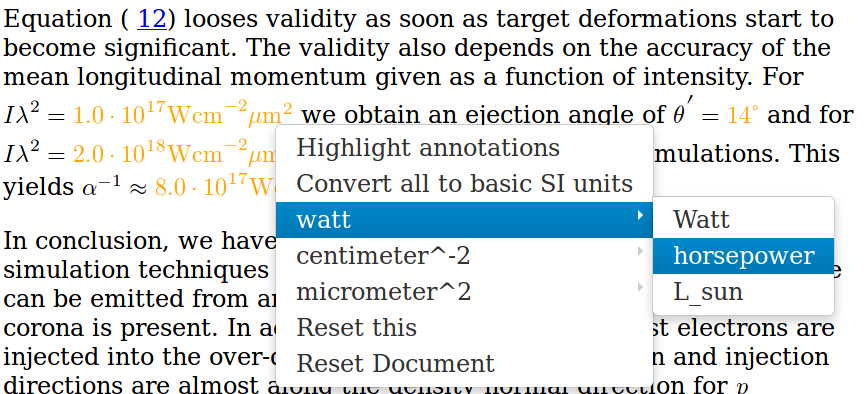
\includegraphics[scale=0.3]{screenshots/convertone.png}
\caption{The user can convert an expression, by choosing the desired
unit from a list of equivalent ones.}
\label{fig:convertone}
\end{figure}

\begin{figure}
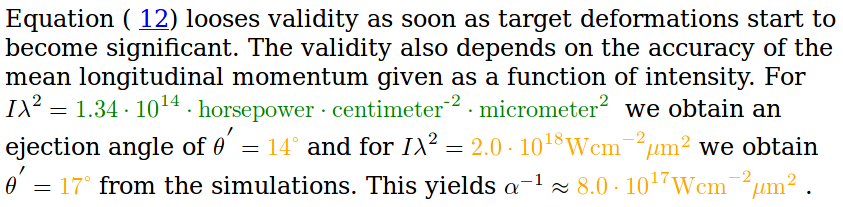
\includegraphics[scale=0.3]{screenshots/convertoneresult.png}
\caption{The result of the computation from Figure~\ref{fig:convertone}. 
The modified quantity expression is highlighted in orange.}
\label{fig:convertoneresult}
\end{figure}

The current example only allows local conversions, but of course the user also wants
to convert units document-wide -- ideally from one system of measurement to another. 
Figure~\ref{fig:si} shows the result of a prototypical implementation, which 
converts all units to irreducible SI base units. 
This could, for instance, be extended to automatically convert all quantity
expressions in a document from imperial to metric units and vice versa. 

\begin{figure}
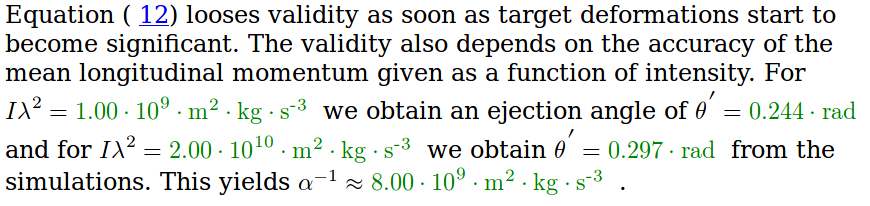
\includegraphics[scale=0.3]{screenshots/si.png}
\caption{All units have been converted to their corresponding SI base units for this example.}
\label{fig:si}
\end{figure}

  


\end{newpart}

%%% Local Variables:
%%% mode: latex
%%% TeX-master: "report"
%%% End:
